\documentclass[pdfcover,bachelor]{scutthesis}
\usepackage{graphicx}
\usepackage{bm}
\usepackage[inline]{enumitem}
\usepackage{wrapfig}
% \usepackage{setspace}

\usepackage[hidelinks]{hyperref}

\hypersetup{pdftitle={数据库的自然语言接口关键技术研究},
	pdfauthor={胡玮文},
	pdfkeywords={深度学习, 自然语言处理, 语义分析, SQL, 自动编程},
	pdfstartview=FitH}

\def\softmax{\mathrm{softmax}}

\begin{document}

\maketitle
\frontmatter
\tableofcontents{}
\begin{abstractCN}
关系型数据库在如今的各种系统中都是不可或缺的一部分。传统上,只有专业人员使用SQL语言与数据库直接交互。而数据库的自然语言接口技术旨在将自然语言表达的查询翻译为SQL语句,允许任何人更方便,更灵活地查询数据。随着基于神经网络的方法近年来在自然语言理解方面的巨大进步,数据库的自然语言接口技术也成为了可能。但还面临一些挑战:1. 如何快速迁移到训练时未曾见过的数据库架构上;2. 如何处理自然语言中的上下文信息;3. 如何有效地将语义信息编码为SQL语句。

本文在现有方法地基础上,进行了一系列改造,并应用了其他研究中最新的预训练模型。特别地,本文提出了关系编码,帮助神经网络更好地理解数据库架构;提出了上下文编码,更好地利用自然语言中的上下文信息;以及提出了新的SQL生成方案,更加高效的生成准确的SQL语句。在最新的富有挑战性的SParC数据集上,相比之前问题完全匹配准确率为47.2\%的最好成绩,本文将其提升至了58.5\%,并大大简化了模型结构。
\end{abstractCN}
\keywordsCN{深度学习;自然语言处理;语义分析;SQL;自动编程}

\begin{abstractEN}
Relational databases are an indispensable part of today's various systems. Traditionally, only professionals can directly interact with databases using SQL language. The natural language interface of the database aims at translating queries expressed in natural language into SQL statements, allowing anyone to query data more conveniently and flexibly. With the tremendous progress of neural network-based methods in natural language understanding in recent years, the natural language interface of databases has also become possible. But some challenges still exists: 1. How to quickly migrate to a database schema that has not been seen during training; 2. How to deal with context information in natural language; 3. How to effectively encode semantic information into SQL statements.

Based on the existing methods, this paper makes a few improvements, and merges in the newest pretrained model from previous research. Especially, this paper proposes relation encoding to help neural networks to better understand the database schema; context encoding is proposed to better use the context of natural language; and a new SQL decoding scheme is proposed to generate accurate SQL statements more efficiently. On the latest and challenging SParC dataset, this paper boosts the question exact match accuracy to 58.5\%, compared to 47.2\% for the previous state-of-the-art model, with a much-simplified model architecture.
\end{abstractEN}
\keywordsEN{Deep Learning, Natural Language Processing, Semantic Parsing, SQL, Automated programing}


\mainmatter

\chapter{绪论}

\section{引言}

当今社会,各行各业都在向信息化的方向飞速发展,数据已经深入到了生活中的点点滴滴。对于专业人员来说,他们可以使用如SQL之类的计算机语言来直接地访问数据库,充分,灵活地表达自己的意图。然而对于大多数普通民众来说,他们对数据的访问依然是十分受限的,只能使用软件厂商预先设计好的用户界面来获取和分析数据。如何能让更广泛的人群更充分地利用海量的数据成为了信息化过程中的一个新的问题。

\section{研究背景}

随着信息化进程的不断加速,大数据时代的到来,数据体量的不断增大,更加突显出了人们在分析利用数据上的瓶颈。近年来自然语言理解上的研究卓有成效,个人语音助理之类的产品也已经走入了千家万户。用户普遍接受使用自然语言来表达自己的意图。开发数据库的自然语言接口正是顺应了这样的趋势。将自然语言的人机交互方式推上了更加正式的场合,将数据库的访问推向了更广阔的用户。如今数据库的自然语言接口的研究集中在将自然语言翻译为现有系统可以执行的指令,如SQL语句。这样的任务也称作自然语言到SQL转换 (Text to SQL) 任务。

新发布的标注数据集包含了自然语言问题和对应的SQL标注,这大大促进了该领域的研究,使得模型可以直接以SQL语句作为监督来训练。与之前的数据集不同,新的数据集,如WikiSQL\cite{seq2sql17}、Spider\cite{spider18}、SParC\cite{sparc19}以及中文数据集CSpider\cite{cspider19}等,在测试时使用训练时未见过的数据库架构,为模型提出了更贴近实际应用的跨领域泛化的挑战。Spider数据集中的数据库架构包含有多个表,且有主键,外键,字段类别等更丰富的结构化信息;SParC数据集则进一步引入了自然语言的上下文信息,允许用户通过多轮对话来补充,更改查询的内容。这些数据集促进了研究向更加实际的场景发展。

跨数据库的泛化能力对模型来说是个不小的挑战。早期研究中的模型是类似机器翻译任务的,直接将自然语言翻译为SQL。在跨数据库的泛化中,模型需要将数据库架构进行编码,得到所有列和表的向量表示以供解码SQL时使用。在编码的过程中,需要精心设计以充分利用数据库架构的名字、类别、主键、外键等信息。另外,模型需要识别自然语言中对数据库中列和表的引用。在不同的领域中,引用的方式也会有所不同。这个识别过程称作架构关联 (Schema linking)。

对自然语言中的上下文的处理也是关键的。实际场景中,对于较复杂的查询,用户通常需要在和系统的交互中不断调整才能完成。用户也可能调整自己的查询来探索数据的不同方面。自然语言的语义是和上下文有很强的关联的,有大量的指代和省略的现象。并且随着用户交互的进行,查询将变得越来越复杂。如何在复杂的查询中依然保持准确也是模型的一个挑战。

对输出SQL的解码工作是十分工程化的。先前的工作已经在这方面做了很多工作。如设计一个能确定性翻译到SQL的中间语言,使用SQL语法限制解码,使用SQL执行结果来指导解码等。虽然如此,但这方面依然有改进的可能:1. 相比自然语言,SQL的语义抽象程度较低,有时需要使用复杂的结构来表达相对简单的语义,之前的中间语言的设计并未完全解决此问题;2. SQL的语法在设计上更考虑的是方便人类编写和读取,对于机器则不是那么适合。

在本文中,我基于SParC数据集上的最佳方法EditSQL\cite{edit19},针对以上各方面进行改进,使得性能有了显著提高。在SParC数据集上达到了58.5\%的完全匹配准确率。

\section{研究现状}

近期新数据集的发布带动了基于语义分析方法的自然语言到SQL转换的研究。最近的研究大都以更加贴近实际的Spider和SParC数据集作为目标。在这些数据集中充分体现了上述困难和挑战。

在编码器的构造上,之前的工作主要分为两类。 \citet{gnn19}提出使用图神经网络 (GNN) 编码数据库架构信息,另外使用LSTM\cite{lstm97}编码自然语言。IRNet\cite{irnet19}使用添加了大量注意力机制的LSTM分别编码自然语言和数据库架构。RAT-SQL\cite{ratsql19}在LSTM生成的表示基础上,使用具有关系感知的自注意力机制的Transformer\cite{attn17}对自然语言和数据库架构进行协同编码。在处理数据库架构中的主键、外键关系时: \citet{gnn19}将这些关系表示为有向图,并用GNN编码它;IRNet忽略了这些关系;而RAT-SQL用自注意力机制编码这些关系。在处理架构链接时:IRNet在输入中添加特殊的“链接类型”嵌入来表达; \citet{gnn19}基于词向量嵌入和一些手工构造的特征来计算自然语言中的单词和数据库列之间的相似度; \citet{gnn19}的后续工作Global-GNN\cite{ggcn19}将自然语言查询的语义信息引入GNN的初始化中;RAT-SQL则将链接关系使用同样的自注意力机制来编码。

在解码器部分,部分研究使用模板填充的方式,将解码过程建模为多分类任务\cite{cao19,seq2sql17,sqlnet17}。
但更多近期的研究将解码过程建模为序列生成任务,它们大多使用了基于LSTM的解码器,主要有基于Token的解码\cite{edit19}和基于抽象语法树的解码\cite{irnet19,gnn19,ggcn19,syntaxsqlnet18}。
IRNet设计了一种比SQL抽象层次更高的语言。还有一些小的改进,如:由粗到细地解码\cite{irnet19,coarse-to-fine18};使用记忆增强的指针网络以减少网络生成重复的内容;使用执行结果来指导解码\cite{wang2018execution-guided},生成后进行额外的辨别步骤等\cite{ggcn19}。

\section{论文结构}

本文分为四章。其中第一章简述了数据库的自然语言接口的研究背景和意义以及自然语言到SQL转换任务的基础知识和研究现状等。第二章节从神经网络的发展历史、网络结构、学习规律三方面详细的讲述了相关神经网络的基础知识。第三章具体定义了本要解决的问题。第四章描述了本文对先前工作各方面的改进方案。第五章节是自然语言到SQL转换实验的结果与分析。

\chapter{神经网络的基础知识}

\section{神经网络的运行原理}

本节中将以最基本的全连接前馈神经网络为例,介绍神经网络的基本运行原理。

训练神经网络是以让神经网络拟合任意的函数为目标的。例如,在图像分类任务中,神经网络输入的是从图片中提取的特征,输出的是该图片是每一分类的得分。训练的目标就是让神经网络输出中正确的一类的得分尽可能高。

神经网络模型的开发过程一般是,搭建模型的结构,然后反复运行前向传播,反向传播,优化这三个步骤,直至收敛。

\subsection{前向传播}

\begin{figure}[]
    \centering
    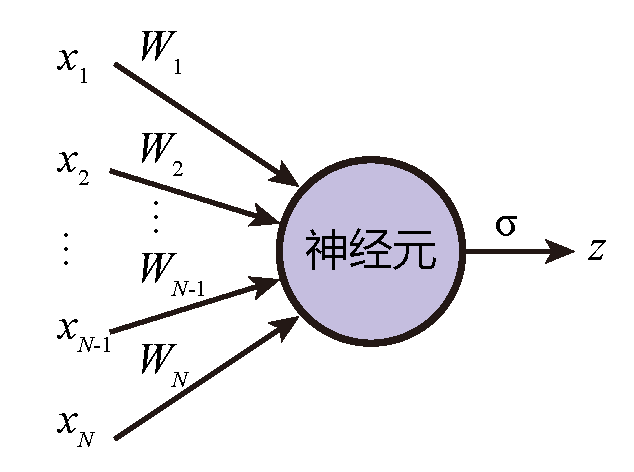
\includegraphics[page=1]{figure/figures.pdf}
    \caption{神经元示意图}
    \label{nunit}
\end{figure}

如图\ref{nunit}所示,神经元是全连接前馈神经网络的基本单元。每个神经元接收若干个信号输入,经过与神经元的权重连接(线性变换)和激活函数(非线性变换)之后,输出一个新的信号。具体来说,神经元接受一个N维向量$\bm{x}\in\mathbb{R}^N$作为输入,则其输出为:

\begin{equation}
    z=\sigma\left(\bm{W}\bm{x}+b\right)
\end{equation}

其中$\bm{W}\in\mathbb{R}^N$是该神经元连接的权重,是可学习的参数。$b$是可选的偏置项,也是可学习的参数,$\sigma$是非线性激活函数。

$M$个接受相同输入的神经元构成了一层神经网络,每个神经元具有不同的可学习参数。则一层神经网络的运行也可以表示为:

\begin{equation}
    \bm{z}=\sigma\left(\bm{W}\bm{x}+\bm{b}\right)
\end{equation}

其中$\bm{W}\in\mathbb{R}^{M\times N}$是该层所有神经元的连接的权重,$\bm{b}\in\mathbb{R}^M$是该层所有神经元的偏置项。$\bm{z}\in\mathbb{R}^M$是该层所有神经元的输出,它可能是模型最后的输出,也可能是下一层神经元的输入。

\begin{figure}[]
    \centering
    \includegraphics[page=2]{figure/figures.pdf}
    \caption{神经网络示意图}
    \label{nnet}
\end{figure}

通常神经网络会由至少三层神经元构成。如图\ref{nnet}所示,第一层称为输入层,其输入是原始的特征向量,最后一层称为输出层,其输出为模型最终的输出,其余的则称为隐藏层,将上一层的输出作为输入,自己的输出则作为下一层的输入。每一层的神经元的数量可以不同。但上一层的神经元数量应和下一层的输入向量的长度是一致的。对于有L层的神经网络来说,若$\bm{x}^0$为表示原始特征的向量,则第l层的输出可以表示为:

\begin{equation}
    \bm{x}^l=\sigma\left(\bm{W}^l\bm{x}^{l-1}+\bm{b}^l\right),l\in\left\{1,2,\ldots,L\right\}
\end{equation}

$\bm{x}^L$即为网络最终的输出。

\begin{figure}[]
    \centering
    \includegraphics{figure/act.pdf}
    \caption{激活函数}
    \label{act-func}
\end{figure}

对于激活函数,理论上它可以是任何连续的非线性函数。若没有激活函数,则整个网络将只有线性变换,无论使用多复杂的结构,输出也只能是输入向量的线性变换,其表达能力十分有限。常用的激活函数有ReLU,tanh,sigmoid等。如图\ref{act-func}所示,以下是它们的定义:

\begin{align}
    \mathrm{ReLU}\left(x\right)&=\max{\left(x,0\right)}\\
    \tanh{\left(x\right)}&=\frac{e^x-e^{-x}}{e^x+e^{-x}}\\
    \mathrm{sigmoid}\left(x\right)&=\frac{1}{1+e^{-x}}
\end{align}

以上介绍的从$\bm{x}^0$计算得到$\bm{x}^L$的过程即为模型的前向传播过程。在前述图像分类任务中,$\bm{x}^L$中即包含了预测的图像属于每一分类的得分。在实际更复杂的神经网络中,在前向传播的过程中可使用任何连续可导的运算,并不局限于上述提到的表达式。

\subsection{反向传播}

反向传播的目的是为网络中的每一个可学习的参数计算一个梯度,当将这些参数的数值向梯度的相反方向移动的时候,我们期望模型在下一次迭代的时候可以做得更好,得出更加正确的结果。为了得到这样的梯度,我们需要一个函数,对模型的输出进行评价,其函数值越小,则代表模型在该任务上的表现越好。这样的函数称作损失函数 (loss function)。我们所期望求得的梯度就是损失函数的梯度了。根据任务的不同,我们会设计不同的损失函数。以之前提到的图片分类任务为例,最常用的损失函数为交叉熵 (cross entropy) 损失函数,其针对单个输入样本的定义为:

\begin{equation}
    \mathrm{CE}\left(\bm{x},y\right)=-\log{\left(\frac{\exp{\left(\bm{x}_y\right)}}{\sum_{j=1}^{N}\exp{\left(\bm{x}_j\right)}}\right)}
\end{equation}

其中$N$为分类的数量,$\bm{x}\in\mathbb{R}^N$为模型输出的各个分类的得分,$y$为正确的分类的下标。正确的分类的得分越高,其他分类的得分越低,该函数的函数值就越小,越趋近于0。
下面以2.1.1节介绍的全连接前馈神经网络中的参数$\bm{W}^l$为例,介绍反向传播的计算过程。其基本思路是函数的链式求导法则。具体来说,我们所要求的梯度是:

\begin{equation}
    \nabla\bm{W}^l=\frac{\partial J\left(\cdot\right)}{\partial\bm{W}^l}
\end{equation}

其中$J\left(\cdot\right)$为损失函数。

在反向传播的过程中,我们从输出层至输入层,反向逐层求解每层的梯度。损失函数的导数将根据损失函数的不同而不同,为讨论方便,我们假设损失函数的偏导数$\frac{\partial J\left(\cdot\right)}{\partial\bm{x}^L}$为已知的。同样地,我们假设激活函数$\sigma$的导数是已知的。一般地,对于第$l$层神经网络,令:
\begin{equation}
    \bm{z}^l=\bm{W}^l\bm{x}^{l-1}+\bm{b}^l
\end{equation}

则:
\begin{align}
    \frac{\partial J\left(\cdot\right)}{\partial\bm{z}^l}&=\frac{\partial\bm{x}^l}{\partial\bm{z}^l}\cdot\frac{\partial J\left(\cdot\right)}{\partial\bm{x}^l}\\
    &=\frac{\partial J\left(\cdot\right)}{\partial\bm{x}^l}\odot\sigma^\prime\left(\bm{z}^l\right)\\
\
    \frac{\partial J\left(\cdot\right)}{\partial\bm{W}^l}&=\left[\frac{\partial J\left(\cdot\right)}{\partial\bm{W}_{ij}^l}\right]_{ij}\\
    &=\left[\frac{\partial\bm{z}_i^l}{\partial\bm{W}_{ij}^l}\cdot\frac{\partial J\left(\cdot\right)}{\partial\bm{z}_i^l}\right]_{ij}\\
    &=\left[\bm{x}_j^{l-1}\cdot\frac{\partial J\left(\cdot\right)}{\partial\bm{z}_i^l}\right]_{ij}\\
    &=\frac{\partial J\left(\cdot\right)}{\partial\bm{z}^l}\cdot\left(\bm{x}^{l-1}\right)^T\\
\
    \frac{\partial J\left(\cdot\right)}{\partial\bm{x}^{l-1}}&=\frac{\partial\bm{z}^l}{\partial\bm{x}^{l-1}}\cdot\frac{\partial J\left(\cdot\right)}{\partial\bm{z}^l}\\
    &=\left(\bm{W}^l\right)^T\cdot\frac{\partial J\left(\cdot\right)}{\partial\bm{z}^l}
\end{align}

其中,$\odot$表示逐元素相乘。$\delta^l=\frac{\partial J\left(\cdot\right)}{\partial\bm{z}^l}$也被称为残差。利用上述公式,我们即可从最后一层开始,计算出每一个$\nabla\bm{W}^l$。

\subsection{梯度下降优化}

当我们为每一个参数在反向传播中计算了梯度之后,需要使用优化算法利用求得的梯度将模型更新到更好的算法。以下以最简单的随机梯度下降 (stochastic gradient descent) 方法为例,并以$\theta^i$表示第i次迭代时模型的所有参数,以$\nabla\theta^i$表示它们的梯度:
\begin{equation}
    \theta^{i+1}=\theta^i-\alpha\cdot\nabla\theta^i
\end{equation}

其中$\alpha$表示学习率,是可以调整的超参数。除了简单的随机梯度下降方法外,还有一些著名的优化算法,如带有动量的随机梯度下降 (stochastic gradient descent with momentum),Adam\cite{Adam14}等。

在实际过程中,从单个训练样例中计算得到的梯度将难以反应整个数据集上的数据分布情况,而如果每次迭代都使用整个数据集的样例计算平均梯度则显得浪费计算资源。所以我们一般在每次迭代时从训练集中选出一小批样例并计算它们的平均梯度,称作小批量梯度下降 (mini-batch gradient descent) 方法。

\section{循环神经网络 (RNN)}

2.1节中描述的全连接前馈神经网络只能处理固定长度的特征。这对于例如图片等数据是没有问题的,图片总是能采样到任何希望的大小。然而对于例如自然语言的输入来说,每次输入的长度都是不一样的,神经网络需要有一种机制来处理变长的输入。循环神经网络就应运而生了。

循环神经网络的输入$\bm{X}=\left\{\bm{x}_1,\bm{x}_2,\ldots,\bm{x}_N\right\}$为长度为$N$的序列,序列中每个元素为一个表示该元素特征的向量,其输出$\bm{Y}=\left\{\bm{y}_1,\bm{y}_2,\ldots,\bm{y}_N\right\}$也是长度为$N$的序列。$N$可以随时改变。以自然语言的文本数据为例,语句中的每个单词可以作为输入序列中的一个元素,其向量表示可以来自预先训练的表示,也可以随机初始化词嵌入向量,并将其随模型一起训练。

\subsection{Vanilla RNN}

\begin{figure}[]
    \centering
    \includegraphics[page=3]{figure/figures.pdf}
    \caption{Vanilla RNN单元}
    \label{vanilla-rnn}
\end{figure}

如图\ref{vanilla-rnn}所示,Vanilla RNN 的前向传播过程与2.1节中描述的全连接前馈神经网络有相似之处,它的前向传播算法如下:
\begin{align}
    \bm{h}_t&=\sigma\left(\bm{W}_{hx}\bm{x}_t+\bm{W}_{hh}\bm{h}_{t-1}+\bm{b}_h\right)\\
    \bm{y}_t&=\bm{W}_{yh}\bm{h}_t+\bm{b}_y
\end{align}

其中$\bm{W}_{hx}\in\mathbb{R}^{h\times x},\bm{W}_{hh}\in\mathbb{R}^{h\times h},\bm{W}_{yh}\in\mathbb{R}^{y\times h},\bm{b}_h\in\mathbb{R}^h,\bm{b}_y\in\mathbb{R}^y$均为可学习的参数,$\bm{h}_t$为第$t$次迭代时的隐藏层状态,$\sigma$为激活函数。它和全连接网络一样,都是由线性变换和激活函数组成。不同的是,RNN在每次迭代中使用相同的权重,这就是它称为“循环”的原因,并且它在每次迭代时还接受新的输入$\bm{x}_t$,这样只需调整迭代的次数就能处理不同长度的输入了。此外,由于网络按顺序接受每个输入,它还能捕获到输入中的时序信息,例如自然语言中每个词语的前后顺序,这样的信息在实际中是非常重要的。

但Vanilla RNN具有梯度消失或爆炸的问题,这会严重阻碍模型学习到合适的权重,特别是难以建模长时间间隔状态之间的依赖关系,因此在实际中并不是很常用。

\subsection{LSTM}

\begin{figure}[]
    \centering
    \includegraphics[page=4,width=\linewidth]{figure/figures.pdf}
    \caption{LSTM单元}
    \label{lstm}
\end{figure}

如图\ref{lstm}所示,长短时记忆 (long short-term memory, LSTM)\cite{lstm97}网络是一种当前使用广泛的RNN网络。LSTM除了拥有Vanilla RNN的处理变长输入,捕获时序关系的优点,还中引入了门控机制来控制信息的累计速度,包括有选择地加入新的信息,并有选择地遗忘之前累计的信息,以此来建模长期的依赖关系。LSTM的前向传播过程较为复杂,如下所示:
\begin{align}
\bm{i}_t&=\sigma\left(\bm{W}_i\ \bm{x}_t+\bm{U}_i\ \bm{h}_{t-1}+\bm{b}_i\right)\\
\bm{f}_t&=\sigma\left(\bm{W}_f\bm{x}_t+\bm{U}_f\bm{h}_{t-1}+\bm{b}_f\right)\\
\bm{o}_t&=\sigma\left(\bm{W}_o\bm{x}_t+\bm{U}_o\bm{h}_{t-1}+\bm{b}_o\right)\\
{\widetilde{\bm{c}}}_t&=\tanh{\left(\bm{W}_c\bm{x}_t+\bm{U}_c\bm{h}_{t-1}+\bm{b}_c\right)}\\
\bm{c}_t&=\bm{f}_t\odot\bm{c}_{t-1}+\bm{i}_t\odot{\widetilde{\bm{c}}}_t\\
\bm{h}_t&=\bm{o}_t\odot\tanh{\left(\bm{c}_t\right)}
\end{align}

其中$\bm{W},\bm{U},\bm{b}$均为可学习的参数,$\sigma$为sigmoid函数。$\bm{i}$为输入门,$\bm{f}$为遗忘门,$\bm{o}$为输出门,$\bm{c}$为记忆单元,$\bm{h}$为输出的隐藏状态。LSTM在记忆单元中保存需要长期保存的信息,并通过输入门控制有多少新的信息进入记忆单元,通过遗忘门控制有多少旧的信息要保留在记忆单元中,并通过输出门控制当前隐藏状态的输出信息。通过广泛使用门控机制,LSTM可以有效避免梯度消失或爆炸的问题。

除上面介绍的两种外,研究者们还提出了一些其他的循环神经网络,如GRU\cite{cho-etal-2014-properties},以及在LSTM基础上的改进等。

\section{注意力神经网络}

长期以来,循环神经网络架构都是处理自然语言数据的唯一选择。Transformer\cite{attn17}提出后,它在一定程度上取代了原来LSTM的地位,在机器翻译等任务上再次取得了突破性的进步。Transformer完全摈弃了循环神经网络的前向传播方法,而是使用注意力机制来建模序列之间的关系,同时使用额外的位置编码来建模序列中的时序信息。它摒弃了循环的结构,因此天生更适合捕获在序列中距离较远的依赖信息,并且可以同时感知序列前后两个方向的上下文。此外,它对每个元素的计算是并行的,这可以更好地利用现代高度并行化的计算硬件,大大提高模型的速度。

\subsection{注意力机制}

\begin{figure}[]
    \centering
    \includegraphics[width=\linewidth]{figure/scaled_multiheaded_attn.png}
    \caption{缩放后的多头注意力机制示意图\cite{attn17}}
    \label{attn}
\end{figure}

如图\ref{attn}所示,缩放后的多头注意力机制是Transformer模型的核心组件,它可以建模任意长度的序列中元素间的关系,允许每个元素在编码过程中访问与自己有关的上下文。这里仅介绍自注意力机制,用于解码的交叉注意力则不做介绍。$\bm{x}$为注意力力机制的输入,$\bm{z}$为输出,其前向传播过程可以表示为:
\begin{align}
    e_{ij}^{\left(h\right)}&=\frac{\left(\bm{W}_Q^{\left(h\right)}\bm{x}_i\right)^T\bm{W}_k^{\left(h\right)}\bm{x}_j}{\sqrt{d_z/H}}\\
    \alpha_{ij}^{\left(h\right)}&=\frac{\exp{\left(e_{ij}^{\left(h\right)}\right)}}{\sum_{l=1}^{n}\exp{\left(e_{il}^{\left(h\right)}\right)}}\\
    \bm{z}_i^{\left(h\right)}&=\sum_{j=1}^{n}{\alpha_{ij}^{\left(h\right)}\left(\bm{W}_V^{\left(h\right)}\bm{x}_j\right)}\\
    \bm{z}_i&=\mathrm{Concat}\left(\bm{z}_i^{\left(1\right)},\ldots,\bm{z}_i^{\left(H\right)}\right)
\end{align}

其中H为注意力头的数量,$\bm{W}$是可学习的权重,$\alpha_{ij}$又称作注意力权重,它编码了第$i$个元素到第$j$个元素的关系紧密程度,具有较强的可解释性。

\subsection{Transformer编码器}

\begin{figure}[]
    \centering
    \includegraphics[page=5]{figure/figures.pdf}
    \caption{Transformer编码器示意图\cite{attn17}}
    \label{trans-enc}
\end{figure}

如图\ref{trans-enc}所示,建立在自注意力机制之上,Transformer编码器交替使用了自注意力层和前馈网络层,并使用了归一化和残差连接。$\bm{y}$表示单层编码器的输出,与公式2-1到2-4一起,其前向传播过程可表示为:
\begin{align}
{\widetilde{\bm{y}}}_i&=LayerNorm\left(\bm{x}_i+\bm{z}_i\right)\\
\bm{y}_i&=LayerNorm\left({\widetilde{\bm{y}}}_i+\bm{W}_2\left(ReLU\left(\bm{W}_1{\widetilde{\bm{y}}}_i\right)\right)\right.
\end{align}

其中$\bm{W}$可学习的是参数,LayerNorm表示层归一化\cite{LayerN16}。$N$个这样的层叠加在一起组成了Transformer的编码器。可以发现,自注意力机制并不能捕获序列中元素的位置信息,而前馈网络层是对每个元素单独运算的,也不能捕获位置信息。因此,Transformer将输入序列中元素的位置信息进行嵌入,并叠加在了首层的输入上。

\section{其他神经网络构建单元}

\subsection{池化层}

池化层之前广泛应用于计算机视觉的网络中,一般用于降低空间维度的大小,以减小计算量,并提升特征的抽象程度。在自然语言处理相关模型中,池化层的使用比较灵活,比如对于自然语言句子中语义相关联的几个单词,或者整个句子,我们希望能得到它们一个全局的向量表示,就可以使用池化层来融合它们的表示。常用的池化层包括平均池化和最大池化。它们的前向传播过程非常简单。若需要池化的区域为R,则前向传播过程如下:
最大池化:
\begin{equation}
    y=\max_{i\in R}{x_i}
\end{equation}

平均池化:
\begin{equation}
    y=\frac{1}{\left|R\right|}\sum_{i\in R}x_i
\end{equation}

其反向传播算法较为特殊,值得特别进行讨论。池化层没有可学习的参数,它仅将梯度反向传播至它的输入层。对于最大池化,它将梯度传递给区域中最大的元素,即:
\begin{equation}
    \frac{\partial J}{\partial x_i}=\begin{cases}
        \frac{\partial J}{\partial y}, & x_i=\max_{j\in R}{x_j}\\
        0, & \mathrm{otherwise}
    \end{cases}
\end{equation}

平均池化则可以使用普通的求导方法,即:
\begin{equation}
    \frac{\partial J}{\partial x_i}=\frac{1}{\left|R\right|}\cdot\frac{\partial J}{\partial y}
\end{equation}

\subsection{嵌入层}

嵌入 (embedding) 层在自然语言相关的模型中非常常用。它能将现实中离散的概念转换成高维空间中的连续的向量。例如,它将自然语言中的每一个单词,或者将分类任务中的类别转换为它的向量表示。嵌入层与其他的神经网络模块不同,它的输入是离散的,这意味着,没有损失函数对输入的导数存在,它不能反向传播到更早的层中。所以嵌入层仅能作为神经网络的第一层。嵌入层的实现非常简单,类似于字典查找,即对于第n种概念,输出矩阵$\bm{W}$的第n行。也可看作是one-hot向量使用矩阵$\bm{W}$进行线性变换。$\bm{W}$是可学习的参数。对于反向传播,则是直接将输出的梯度传播到$\bm{W}$中被选中的行,其它行的梯度则为0。

\section{本章小结}

本章介绍对神经网络的运行原理:前向传播,反向传播,优化方法进行了介绍。并介绍了在自然语言相关任务中最常使用的神经网络模块:全连接前馈神经网络,循环神经网络和注意力神经网络,以及其他一些辅助模块。这些介绍也反应了神经网络在这一领域的发展历史。这些原理和模块也是后文构建方案的基础。

\chapter{跨领域上下文相关语义分析}

\section{数据集} \label{dataset}

本文主要使用最新的SParC\cite{sparc19}数据集作为主要的性能指标。它是一个大规模的,上下文相关的,具有SQL标注的语义分析数据集。

SParC数据集和之前的数据集相比有一些显著的不同。SParC数据集是基于Spider\cite{spider18}数据集构建的。Spider数据集是不包含上下文的,其中一个例子仅包含一个问题和一个SQL标注。相比于Spider数据集,SParC数据集中的每一次交互都是以Spider数据集中的一个问题作为交互目标,标注者被要求询问几个相互关联的问题来获取信息以完成该目标。其平均每次交互的轮数约为3.0轮。ATIS数据集是早些时候被广泛研究的数据集,但它所有的例子都是限制在一个领域之内的,所有交互使用同样的数据库架构。而在SParC数据集中总共包括了200个不同的数据库架构,且在测试时使用的数据库架构都是没有在训练集中出现的。这要求模型能够在推理阶段适应不同的领域。另外,SParC数据集中的问题和SQL语句也显著复杂于ATIS数据集,有些问题还需要一定的生活常识才能正确解答。

作为总结,我们之所以选择SParC数据集是因为它对模型提出了新的,更接近实际的挑战:1. 包含更复杂的自然语言上下文依赖关系;2. 覆盖了更多,更复杂的语义;3. 使用了跨领域的设置。

\section{问题定义}

定义$X$为自然语言语句,$Y$为对应的SQL查询语句,在一次用户交互$I$中,包括$n$个交互回合:$I=\{\langle X_i,Y_i\rangle\}_{i=1}^n$。定义数据库架构$T=C,T,R$,其中包含数据表列$C=\left\{c_1,c_2,c_3,\ldots,c_{\left|C\right|}\right\}$,每一个列名$c_i$包含单词$c_{i,1},\ldots,c_{i,\left|c_i\right|}$。包含数据表$T=\left\{t_1,t_2,t_3,\ldots,t_{\left|T\right|}\right\}$, 每一个表名$t_i$包含单词$t_{i,1},\ldots,t_{i,\left|t_i\right|}$。$T$中也包含主键,外键等关联信息,标记为$R$。在第$t$个交互回合,模型的目标是输入$T$,$X_t$和交互历史记录$\{\langle X_i,Y_i\rangle\}_{i=1}^{t-1}$,并生成$Y_t$。

\chapter{自然语言到SQL转换方案设计}

\begin{figure}
    \centering
    \includegraphics[page=6,width=\linewidth]{figure/figures.pdf}
    \caption{模型整体架构}
    \label{arch}
\end{figure}

在整体架构上,本文使用的是带有注意力机制的编码器-解码器模型,如图\ref{arch}所示。这个框架主要包括了:1. 自然语言与数据库架构编码器,它对自然语言的查询和数据库架构进行协同地编码;2. SQL解码器,它同时考虑自然语言查询,数据库架构和之前交互中的SQL语句,做出决策,逐个标记地生成SQL查询语句。

\section{数据预处理和后处理}

本文在将SQL输入给网络进行训练时先进行了预处理。SQL是人工设计的产物,其具有严格的语法,可以在抽象语法树的层面进行具体的分析和编辑操作。注意到在SQL语句中,由于历史原因,或者是语义准确性的考虑,通常包括了一些繁琐的,抽象程度较低的部分。这些部分将不必要地给SQL的生成带来困难。本文试图将这些繁琐的部分去除,再在SQL生成后确定性地恢复这些内容。

在最终使用的方案中,本文进行了如下的预处理:
\begin{enumerate}
    \item 去除所有JOIN子句中的ON部分。
    \item 去除FROM子句中用于多对多关联的JOIN子句
    \item 在FROM子句中,去除所有在SQL的其他部分引用过的表。若所有表都被去除,则去除整个FROM子句。
\end{enumerate}

在后处理过程中,本文使用以下方法试图恢复这些内容:
\begin{enumerate}
    \item 将所有在SQL中引用过的表添加到FROM子句中。
    \item 根据外键关系,将数据库中的所有表构造成无向图,并使用Kruskal算法求解包含当前FROM子句中的表的最小生成树,根据生成树的边来重建JOIN子句中的ON部分。该步骤也有可能会添加新的表至FROM子句中,例如用于多对多关联的表。构建最小生成树也可能失败,例如数据库架构的外键约束不完整时。若构建失败,则跳过重建JOIN子句ON部分。
\end{enumerate}

\begin{table}
    \def\sql#1{\texttt{#1}}
    \def\kw#1{\textcolor{blue}{#1}}
    \def\SELECT{\kw{SELECT }}
    \def\FROM{\kw{FROM }}
    \def\JOIN{\kw{JOIN }}
    \def\AS{\kw{AS }}
    \def\ON{\kw{ON }}

    \begin{tabularx}{\textwidth}{l|X}
    \hline
    自然语言查询 & Who are all the party hosts?…\newline Show the themes of parties they host along with their name.\\ \hline
    原SQL语句 &
    \sql{\SELECT T3.Party\_Theme, T2.Name \FROM party\_host \AS T1 \newline
        \-\hspace{2em} \JOIN host \AS T2 \ON T1.Host\_ID = T2.Host\_ID \newline
        \-\hspace{2em} \JOIN party \AS T3 \ON T1.Party\_ID = T3.Party\_ID} \\ \hline
    预处理后SQL语句 &
    \sql{\SELECT party.Party\_Theme, host.Name} \\ \hline
    \end{tabularx}
    \caption{SQL预处理。party\_host是多对多关联表,host和party表均在SELECT子句中被引用过,所以整个FROM子句全部被去除。}
    \label{preprocess-eg}
\end{table}

表\ref{preprocess-eg}展示了一个预处理的示例。在将SQL输入神经网络前需要将它分割为多个标记。本文使用的分割方法基本思路为将一个关键字、运算符分为一个标记,将对数据库中列或表的引用的表达式视作一个整体,分为一个标记,并与其引用的列或表相关联。有部分关键字总是一同出现,例如GROUP BY等,则将它们视作整体,分为一个标记。在对数据库中列或表的引用的表达式中可能出现多个标识符,别名等。本文对各种情况都手动进行解析,将其关联到它真正引用的表或列。例如表 4 1中的SQL语句最终被分为4个标记。

对于自然语言查询的预处理,本文使用了匹配预训练的预处理方法。例如,当使用XLNet\cite{XLNet19}预训练模型时,使用SentencePiece对语句进行分词,并使用预训练的词嵌入等。

\section{编码器的设计}

编码器的构建是基于大型预训练注意力神经网络,如BERT\cite{bert19}和XLNet\cite{XLNet19}等。本文在之前工作的基础上增加了关系编码机制和上下文编码机制。

\begin{figure}
    \centering
    \includegraphics[page=7,width=\linewidth]{figure/figures.pdf}
    \caption{编码器架构}
    \label{enc-arch}
\end{figure}

如图\ref{enc-arch}所示是编码器的整体架构。在输入预训练模型之前,本文在数据库架构部分加入了一些特殊的标记帮助模型分隔各数据库列,并提供额外的上下文信息。预训练模型将为每个输入标记输出一个向量表示,这些特殊标记所对应的输出向量表示将被舍弃。在预训练模型输出的向量表示的基础上,自然语言查询的部分再额外使用一个Bi-LSTM\textsuperscript{E}编码,得到所有单词的最终向量表示$\bm{h}^\mathrm{E}$,将Bi-LSTM\textsuperscript{E}正向和反向的最终隐藏状态拼接,得到整个自然语言查询的向量表示$\bm{c}_t^{turn}$,该向量将作为解码器的初始向量,在后文将详细介绍。对于数据库的列名,分别对每个列名中的多个单词使用Bi-LSTM\textsuperscript{C}编码,并将正向和反向的最终隐藏状态拼接,得到每个列的向量表示$\bm{h}^\mathrm{C}$。

\subsection{上下文编码机制}

上下文编码机制非常简单,但十分高效。它将本轮的自然语言查询和本次交互历史中的查询串联起来,再输入到预训练的编码器中。在之前的工作(如EditSQL\cite{edit19})中,通常使用一个额外LSTM构成的“交互编码器”,以及额外的注意力机制来处理自然言语中的上下文信息。而本文认为,预训练的编码器已经在大规模的语料上进行了无监督训练,其训练预料包含了较长的文本段落。从注意力可视化\cite{attn17}中能够得知,在预训练过程中模型已经能一定程度上掌握理解自然语言上下文的能力,例如理解语言中省略,指代的语义。因此,将上下文信息按照匹配预训练的方法,直接串联起来,输入到预训练编码器中是高效的。

\subsection{关系编码机制}

预训练的编码器最初是为机器翻译等任务而构造的,在设计上它处理的是没有明确结构的自然语言文本信息。而在本任务中我们还需要将高度结构化的数据库架构进行编码。与预训练中包含较长文本段落的预料不同,数据库架构是由表名、列名组成,它们都是短小的词或词组,且不包括完整的语法结构,这可能对编码器编码出高效的数据库架构向量表示造成困难。另外,现有的预训练编码器无法利用数据库架构中的例如主键、外键等关系,缺少这些信息显然将增大该任务的难度。

本文提出的关系编码机制在思想上类似于RAT-SQL\cite{ratsql19}中使用的“关系感知的自注意力” (relation-aware self-attention) 机制,但在具体的做法上有所差异。特别地,本文将该机制融合到了预训练的编码器中。以XLNet为例,下面介绍该机制的具体做法:

关系编码发生在编码器的自注意力层。在通常的理解中,每个自注意力头编码了一种学习到的关系,关系的强度被编码在注意力权重$\alpha_{i,j}^{\left(h\right)}$中。XLNet中的自注意力层使用了“相对位置嵌入”(relative positional embedding) 机制,用以代替最初Transformer中提出的位置嵌入。该机制将公式\ref{attn-forward:1}和\ref{attn-forward:2}替换为:
\begin{equation}
    \alpha_{i,j}^{(h)}=
        \left(\bm{W}_Q^{(h)}\bm{x}_i\right)^T\bm{W}_{k,E}^{(h)}\bm{x}_j+
        \left(\bm{W}_Q^{(h)}\bm{x}_i\right)^T\bm{W}_{k,R}^{(h)}\bm{R}_{i-j}+
        \bm{u}^T\bm{W}_{k,E}^{(h)}\bm{x}_j+
        \bm{v}^T\bm{W}_{k,R}^{(h)}\bm{R}_{i-j}
\end{equation}

其中$\bm{W},\bm{u},\bm{v}$是可学习的参数,$\bm{R}_{i-j}$是使用sinusoid计算的相对位置嵌入,不包含可学习的参数。上述公式中的4项可分别理解为
\begin{enumerate*}
    \item 基于内容的寻址;
    \item 内容相关的位置偏好;
    \item 全局的内容相关偏好;
    \item 全局的位置相关偏好。
\end{enumerate*}
这样的设计是为注意力机制提供了有关相对位置信息的线索,这为模型利用各元素间的位置关系提供了可能。类似地,本文提出的关系编码旨在为注意力机制提供有关已经存在的关系的线索,例如数据库架构中的主键、外键等。在训练过程中,模型可以有选择地利用这些线索学习到如何利用已知的关系。为达成此目标,本文在上述4项的基础上再增加两项:
\begin{equation}
    \alpha_{i,j}^{(h)}=\ldots+
        \left(\bm{W}_Q^{(h)}\bm{x}_i\right)^T\bm{W}_{k,R}^{(h)}\bm{T}_{ij}+
        \bm{t}^T\bm{W}_{k,R}^{(h)}\bm{T}_{ij}
\end{equation}

\begin{table}
    \begin{tabularx}{\linewidth}{ll|l|l}
    \hline
    x类型 & y类型 & 关系类型              & 描述                 \\ \hline
    表   & 表   & self-table        & 同一表名中的多个单词         \\
    列   & 列   & self-column       & 同一列名中的多个单词         \\ \hline
    列   & 表   & primary-key       & 列x是表y的主键           \\
    列   & 表   & column            & 列x属于表y,但不是主键       \\
    表   & 列   & table             & 表x包含列y             \\
    列   & 列   & sibling-column    & 列x与y属于同一张表         \\ \hline
    列   & 列   & one-to-many-FK    & 列x与y间有一对多的外键关系     \\
    列   & 列   & many-to-one-FK    & 列x与y间有多对一的外键关系     \\
    表   & 表   & one-to-many-table & 表x与y间至少有一组一对多的外键关系 \\
    表   & 表   & many-to-one-table & 表x与y间至少有一组多对一的外键关系 \\ \hline
    列   & 表/列 & other-column      & 列x与y无特殊关系          \\
    表   & 表/列 & other-table       & 表x与y无特殊关系          \\ \hline
    任意  & 任意  & none              & 其他不表示列名或表名的标记      \\ \hline
    \end{tabularx}
    \caption{为数据库架构设计的,用于关系编码中的关系描述。任何两个输入的标记间都有且只有一种关系成立。}
    \label{rel-def}
\end{table}

类似地,这两项分别可理解为内容相关的关系偏好,和全局的关系偏好。其中$\bm{T}_{ij}$表示元素$i$与$j$之间的关系的嵌入,它被初始化为0,这样在训练初期不会对预训练模型产生干扰。为充分表示数据库架构之间的关系,本文总共设计了13种不同的关系,如表\ref{rel-def}所示。

在基于BERT的模型中,本文也类似地实现了关系编码机制。

\section{解码器的设计}

本文使用的解码器是EditSQL\cite{edit19}中的解码器的重新实现。这是一个基于LSTM的,带有注意力机制和编辑机制的解码器。它可以结合之前的SQL语句,当前的自然语言查询和数据库架构,逐个标记地以自回归的形式进行解码。

\subsection{SQL语句编辑机制}

如\citet{edit19}介绍的,在用户和和系统交互的过程中,倾向于询问一系列紧密相关的问题。需要生成的SQL语句通常和上一轮交互中的SQL语句是有很大部分是重叠的。随着交互的不断进行,SQL语句会越来越复杂,其平均长度会越来越长,但也有更多的标记是和之前的query重叠,需要新增的标记数量是比较稳定的。

基于这样的观察结果,EditSQL\cite{edit19}在解码器中加入了SQL语句编辑机制。具体实现包括在上下文向量中加入了上一语句的信息,以及在输出层中加入了拷贝开关,并增加了拷贝的标记的输出路径,具体将会在下文介绍。

\subsection{解码器具体实现}

在解码的第k步骤中,将解码得到的SQL语句标记嵌入$\bm{q}_k$和上下文向量$\bm{c}_k$相连作为LSTM的输入:
\begin{equation}
    \bm{h}_{k+1}^\mathrm{D}=\mathrm{LSTM^D}\left(\left[\bm{q}_k;\bm{c}_k\right],\bm{h}_k^\mathrm{D}\right)
\end{equation}

其中$\bm{h}^\mathrm{D}$是解码器LSTM\textsuperscript{D}的隐藏状态,$\bm{h}_0$初始化为编码器的状态$\bm{c}_t^{turn}$,当解码得到的标记是一个SQL关键字的时候,$\bm{q}_k$是一个可学习的关键字的嵌入,当它是一个列名的时候,$\bm{q}_k$则是由编码器输出的,该列的向量表示。

上下文向量$\bm{c}_k$包含了解码器隐藏状态到自然语言、数据库架构中列的向量表示和上一次的SQL语句的注意力。解码器隐藏状态到数据库列的注意力可表示为:
\begin{align}
    \bm{s}_l&=\bm{W}_\mathrm{column-att}\bm{h}_k^\mathrm{D}\cdot\bm{h}_l^\mathrm{C}\\
    \bm{\alpha}^\mathrm{column}&=\softmax\left(\bm{s}\right)\\
    \bm{c}_k^\mathrm{column}&=\sum_{l}{\bm{\alpha}_l^\mathrm{column}\times\bm{h}_l^\mathrm{C}}
\end{align}

其中,$\bm{h}_l^\mathrm{C}$为数据库中第$l$列的向量表示。解码器隐藏状态到自然语言的注意力可表示为:
\begin{align}
    \bm{s}_i&=\bm{W}_\mathrm{utterance-att}\bm{h}_k^\mathrm{D}\cdot\bm{h}_i^\mathrm{E}\\
    \bm{\alpha}^\mathrm{utterance}&=\softmax\left(\bm{s}\right)\\
    \bm{c}_k^\mathrm{utterance}&=\sum_{i}{\bm{\alpha}_i^\mathrm{utterance}\times\bm{h}_i^\mathrm{E}}
\end{align}

其中$\bm{h}_i^\mathrm{E}$为拼接后的当前和历史记录中的自然语言查询中的第i个单词的向量表示。类似地,解码器隐藏状态到上一次的SQL语句的注意力可表示为:
\begin{align}
    \bm{s}_i&=\bm{W}_\mathrm{query-att}\bm{h}_k^\mathrm{D}\cdot\bm{h}_i^\mathrm{Q}\\
    \bm{\alpha}^\mathrm{query}&=\softmax\left(\bm{s}\right)\\
    \bm{c}_k^\mathrm{query}&=\sum_{i}{\bm{\alpha}_i^\mathrm{query}\times\bm{h}_{t-1,i}^\mathrm{Q}}
\end{align}

其中,$\bm{h}_{t-1,i}^\mathrm{Q}$表示上一个SQL语句中的第i个标记的向量表示。这个表示是由另一个LSTM编码得到的,上下文向量是由上述三者连接在一起得到:
\begin{equation}
    \bm{c}_k=\left[\bm{c}_k^\mathrm{column};\bm{c}_k^\mathrm{utterance};\bm{c}_k^\mathrm{query}\right]
\end{equation}

在输出层中,模型通过当前LSTM的隐藏状态$\bm{h}_k^\mathrm{D}$和上下文向量$\bm{c}_k$,做出SQL语句解码的决策,其决策分为三个分支:1. 解码一个SQL关键字 (SELECT, WHERE等);2. 解码一个数据库表或者列;3. 从上一个SQL语句中拷贝一个标记。在跨领域的设定中,每次解码时SQL关键字都是一样的,而数据库架构则不同,所以使用不同的模块来解码两者是非常关键的。在拷贝的分支中,我们预测了一个独立的开关来控制是否需要拷贝。最终,使用softmax来综合各个分支,并获取生成标记的概率分布。
\begin{equation}
    \bm{o}_k=\tanh{\left(\bm{W}_o\left[\bm{h}_k^D;\bm{c}_k\right]\right)}
\end{equation}
拷贝开关预测:
\begin{align}
    p_\mathrm{copy}=\sigma\left(\bm{W}_\mathrm{copy}\bm{o}_k+b_\mathrm{copy}\right)\\
    p_\mathrm{gen}=1-p_\mathrm{copy}
\end{align}
对于拷贝分支概率分布,$\bm{P}_\mathrm{prevSQL}$表示在上一SQL语句中每个标记复制到当前位置的概率:
\begin{align}
    \bm{P}_\mathrm{prevSQL}=\softmax\left(\bm{W}_\mathrm{prevSQL}\bm{o}_k\cdot\bm{h}_{t-1}^Q\right)
\end{align}
对于生成分支概率分布,$\bm{P}_\mathrm{gen}$表示生成任何可能的标记的概率:
\begin{align}
\bm{m}_{SQL}=\bm{W}_{SQL}\bm{o}_k+\bm{b}_{SQL}\\
\bm{m}_{column}=\bm{W}_{column}\bm{o}_k\cdot\bm{h}^C\\
\bm{P}_\mathrm{gen}=softmax\left(\left[\bm{m}_{SQL};\bm{m}_{column}\right]\right)
\end{align}
最终决策的生成下一个标记的概率分布为:
\begin{align}
p\left(y_k^t\right)=p_\mathrm{copy}\sum_{l\in\left\{l|y_l^{t-1}=y_k^t\right\}}{\bm{P}_\mathrm{prevSQL}\left(y_l^{t-1}\right)}+p_\mathrm{gen}\cdot\bm{P}_\mathrm{gen}(y_k^t)
\end{align}
其中,$\bm{P}_\mathrm{gen}(y_k)$表示生成$y_k$标记的概率,$\sum_{l\in\left\{l|y_l^{t-1}=y_k^t\right\}}{\bm{P}_\mathrm{prevSQL}\left(y_l^{t-1}\right)}$表示在上一SQL语句中,所有出现的$y_k$标记的复制概率之和。当一次交互中的首个SQL语句解码时,不存在上一个SQL语句,这时将$p_\mathrm{copy}$设为0并跳过拷贝分支。注意到对于所有可能的$y_k$,$p\left(y_k\right)$之和将仍为1,无需进一步归一化。

\section{本章小结}

本章详细介绍了实现自然语言到SQL转换任务的方案,这是一个端到端的神经网络。其中相对于之前的工作,有以下创新:使用适当的SQL预处理和后处理过程,帮助网络高效的生成准确的SQL语句;加入上下文编码机制,帮助网络更好地理解自然语言上下文;在预训练模型中加入关系编码机制,能将预定义的主键,外键等信息编码,并指导自注意力机制,提升编码质量。

\chapter{实验结果及分析}

\section{评价指标}

如\ref{dataset}节所述,本文使用主要使用最新的SParC数据集作为性能指标。我们使用预测的和标注的SQL语句间的“完全集合匹配精确度”。为避免不影响SQL语义的顺序问题,跟随 [3]中的做法,我们并不使用简单的字符串匹配方法,而是将SQL分解为多个子句,并对每个子句分别按照语义进行忽略顺序的“集合匹配”。本文主要报告两种指标:问题准确率,按照SQL语句统计,对所有交互中的每个SQL语句分别判断是否匹配;交互准确率,按交互统计,仅整个交互中所有查询均匹配才将该交互计算为匹配。

\section{基线方法}

目前SParC数据集上的工作较少。本文主要与EditSQL进行比较,这是截至2020年5月20日已发布论文的模型中效果最好的。与所有提交的模型相比,其排名也很靠前。本文使用了与其相同的解码器算法,但在其他诸多方面做出了改进。EditSQL在编码器方面,使用了多层的LSTM。为了解决跨领域问题,它设计了较为复杂的自然语言和数据库架构间的交叉注意力机制。另外,它使用了独立的交互编码器和交互注意力机制来处理自然语言上下文的问题。

此外,本文也与SParC\cite{sparc19}中发布的两个基线模型进行比较:上下文相关的序列到序列模型 (Context-dependent Seq2Seq) ,它在原始的为ATIS数据集开发的模型基础上新增了使用Bi-LSTM编码数据库架构的能力,和解码未在训练中见过的数据库架构的能力,以适应跨领域的任务。以及SyntaxSQL-con模型,它在原始的为Spider数据集开发的SyntaxSQL\cite{yu-etal-2018-syntaxsqlnet}模型的基础上增加了Bi-LSTM编码交互历史记录的能力,以适应多轮交互的任务。

\section{实现细节}

本文的模型使用PyTorch\cite{pytorch19}实现。在预训练模型上,由于资源限制,本文仅使用了BERT-base或XLNet-base模型。跟随EditSQL的做法,所有LSTM层的隐藏层的维度为300,编码器的LSTM使用1层,解码器的LSTM则使用2层。本文使用了Adam\cite{Adam14}优化器来优化解码的标记的概率分布上的交叉熵损失函数。对于预训练的模型部分,我们使用1e-5的恒定学习率,其他的模型参数初始学习率定为$1e^{-3}$。在5个epoch后,每个epoch学习率递减到上个epoch的0.85。非预训练的参数使用均匀分布$U\left[-0.1,0.1\right]$初始化,除了关系编码使用的参数,它们初始化为0以避免对预训练模型的干扰。训练在模型连续10个epoch未能提升准确率后停止。通常训练在20个epoch左右收敛。

\section{总体结果}

\begin{table}[]
    \centering
    \caption{SParC实验总体结果}
    \begin{tabular}{lrr}
    \hline
                        & 问题准确率 & 交互准确率 \\ \hline
    SyntaxSQL-con       & 18.5  & 4.3   \\
    CD-Seq2Seq          & 21.9  & 8.1   \\
    EditSQL with   BERT & 47.2  & 29.5  \\
    本文模型 with BERT      & 54.3  & 34.6  \\
    本文模型 with XLNet     & 58.5  & 39.6  \\ \hline
    \multicolumn{3}{l}{使用标注的历史SQL查询}    \\ \hline
    EditSQL with   BERT & 53.4  & 29.2  \\
    本文模型 with BERT      & 60.7  & 34.6  \\
    本文模型 with XLNet     & 64.3  & 39.3  \\ \hline
    \end{tabular}
    \label{overall-results}
\end{table}

表\ref{overall-results}展示了本文在SParC数据集上的结果。本文的方法不仅大幅超过了基线模型SyntaxSQL-con和CD-Seq2Seq,而且还显著优于更为复杂的EditSQL模型,达到了58.5\%的问题准确率和39.6\%的交互准确率,分别比EditSQL提升了11.3\%和10.1\%。这归功于本文中的各项改进,包括上下文编码机制、关系编码机制、新的SQL预处理与后处理,以及更新的预训练模型,后文将具体分析。

为了更公平地与基线方法比较,本文也报告了基于BERT模型的结果。但使用更新的XLNet预训练模型有以下好处:1. XLNet使用更大的预料库,其预训练方法也有较大不同,它或许能生成更好的向量表示;2. BERT由于使用预训练的位置嵌入,其位置嵌入最大值为512,将无法完整容纳较大的数据库架构。之前的工作通过将数据库架构在批维度拆分以解决该问题。本文放弃对数据库架构部分使用位置嵌入,转而完全依赖关系编码机制,从而绕过了这个限制,使得BERT的表现略有提升。而XLNet对输入序列的长度没有限制,所以没有类似的问题。从最终结果看,XLNet也取得了更佳的结果。

\begin{figure}[]
    \centering
    \includegraphics[width=\linewidth]{figure/overall.pdf}
    \caption{SParC实验结果按照交互回合和难度细分。EditSQL使用BERT版本,本文的模型使用XLNet的版本。}
    \label{result-subdivide}
\end{figure}

为了更好地了解模型在用户交互过程中的表现,图\ref{result-subdivide}(左)展示了按照交互轮数细分的指标。随着交互轮数的增加,预测出正确的SQL语句将越来越困难,这是因为自然语言上下文的增长,以及SQL语句本身的复杂度的增加。本文的方法大幅提升了在交互回合数较多时的准确率,特别地,在第四或更多回合时,本文将准确率从19.1\%提升至了48.4\%。类似地,图\ref{result-subdivide}(右)展示了按照难度等级细分的指标。本文的模型在更难的语句中取得的提升更加明显。

\section{消融实验}

\subsection{SQL预处理与后处理效果}

本文进一步研究了SQL预处理和后处理对实验效果的影响。由于SQL具有严格的语法,预处理可操作的范围较广。但本文的研究集中在FROM子句中,因为通常FROM子句是繁琐重复的。

EditSQL也进行了SQL预处理,但没有对此进行讨论。EditSQL的预处理方案是简单地去除整个FROM子句,该方案后文称为“无FROM”。这样的预处理方案虽然能有效提升效果,但有很明显的不足之处:FROM子句中的信息并非都是可以还原的,使用“无FROM”方案预处理过后,将有17.3\%的语句无法通过配套的后处理还原。

本文使用的方案称为“FROM未引用表”,该方案则有效地缓解了这一问题,通过在FROM子句中依然保留一些最有价值的信息,使得仅有2.3\%的语句无法在后处理中还原,余下的无法还原的原因包括:数据集中标注的外键不完整,同一个表参与JOIN多次,使用多个键进行的JOIN等。这些问题难以在当前预处理框架中解决。

同时,本文还对比了一些其他预处理方案:
\begin{itemize}
    \item FROM所有表:简单的在FROM子句中去除所有JOIN,保留所有表名。
    \item FROM未在SELECT中引用的表:类似于“FROM未引用表”,但保留所有未在SELECT子句中引用的表。
    \item SELECT提示:去除整个FROM子句,但将未在SQL其他部分引用的表以特殊标记的形式添加到SELECT子句中。
\end{itemize}

\begin{figure}[]
    \centering
    \includegraphics{figure/preprocess.pdf}
    \caption{各种预处理方案对比。在EditSQL的基础上实验不同的预处理方案。图中误差线展示了基于7次实验估计的95\%置信区间}
    \label{preprocess-results}
\end{figure}

图\ref{preprocess-results}展示了各种方案的实验结果。从结果中可以看到,本文使用的“FROM未引用表”效果最佳,而“FROM所有表”方案的效果最差,甚至低于“无FROM”方案。可见,虽然“无FROM”方案有明显丢失信息的问题,但它对提升该任务的效果依然是有积极意义的。对比“FROM所有表”,“FROM未在SELECT中引用的表”和“FROM未引用表”三个方案,其包含的冗余信息依次减少,效果依次上升,这可以解释为网络并不能很好地理解这些信息是冗余的,当要处理的信息越多时,网络出错的概率也就越高。

\subsection{上下文编码机制效果}

\begin{figure}[]
    \centering
    \includegraphics{figure/prefix.pdf}
    \caption{上下文编码消融实验结果,按交互回合细分}
    \label{context-results}
\end{figure}

本文对上下文编码机制的效果进行了消融实验,表\ref{ablation-results}展示了实验结果。此外,将本文提出的上下文编码机制和EditSQL中使用的“交互编码器”进行对比,并将指标按照交互轮数细分展示,如图\ref{context-results}所示。上下文编码机制能帮助网络更好地理解自然语言的上下文信息。整体上,上下文编码机制使准确率提升了4.3\%。其提高在于第二回合及以后的交互中,也就是所有需要处理上下文信息的回合。

\subsection{关系编码机制效果}

\begin{table}[]
    \centering
    \caption{消融实验结果}
    \begin{tabular}{lrr}
    \hline
            & 问题准确率 & 交互准确率 \\ \hline
    本文模型    & 58.5  & 39.6  \\
    - 上下文编码 & 54.2  & 33.9  \\
    - 关系编码  & 57.1  & 38.9  \\ \hline
    \end{tabular}
    \label{ablation-results}
\end{table}

本文也对关系编码机制的效果进行了消融实验。表\ref{ablation-results}中展示了是否使用关系编码机制的效果对比,结果显示关系编码机制能使效果有小幅提升。RAT-SQL\cite{ratsql19}中也报告了类似的机制,在它们的实验中,关系编码带来的提升很大,而本文的提升幅度有限。本文推测原因可能是,在预训练的网络中,网络已经足够强,而能通过内容自行归纳出一些关系,使得额外编码的关系提升有限。另一可能的解释为,由于已经进行了预训练,网络不能充分利用新编码的关系。

\section{错误分析}

\begin{figure}[]
    \centering
    \includegraphics{figure/error.pdf}
    \caption{预测错误分析}
    \label{error}
\end{figure}

本文对模型预测错误的语句进行了分析,具体方法是将预测的SQL语句和标注的SQL语句分别转换成抽象语法树,并对语句的各个部分进行对比,结果如图\ref{error}所示。尽管在解码时没有使用SQL的语法进行约束,解码的结果只有很少量的语法错误,其中大多数是括号不匹配等错误。这可能说明模型对SQL的语法已经能较好地掌握了。对于包含组合和子查询的复杂语句模型还较难处理,模型仅正确预测出了39个组合结构中的7个(18\%),和75子查询结构中的42个(56\%)。鉴于巨大的搜索空间和很少的训练数据,这是可以理解的。但测试数据较少,所以这类错误总量也较少。绝大多数错误都来自单个子查询内的错误。其中较高层次的骨架错误和较低层次的列选择错误都有较高的比例,这意味着对于未来的研究来说,各个层次都是很重要的。由于本文特别对FROM子句部分进行了预处理,所以也特别分析了FROM子句的错误情况。在经过预处理之后,相对来说,FROM子句造成的错误是比较少的。

\section{本章小结}

本章中介绍了本文提出的模型在SParC数据集上的实验结果,得益于本文提出的各项改进,本文的效果显著超过了目前在该任务上的最佳模型。本章还对本文提出的各种改进进行了消融实验,验证的它们各自的效果。本章还对模型的错误进行了分析,这将帮助未来的工作确定方向。

\chapter{结论}

\section{论文工作总结}

尽管在自然语言到SQL转换任务上已经有了不少研究,但考虑自然语言上下文的研究依然较少。本文提出的简单的上下文编码机制能与预训练模型良好结合,明显提升模型处理上下文的效率。本文提出的新的SQL预处理与后处理方法尽管较简单,但能有效降低SQL中的冗余信息,提升模型解码SQL语句的效率,最终提升任务效果。本文提出的关系编码机制能有效将预定义的关系融入到预训练的模型中。

在实践上,融入了以上改进,并受益于最新的预训练模型,本文的模型在SParC数据集上显著超过了之前最佳的结果。在构建贴近实际的数据库的自然语言接口的过程中更进了一步。

\section{工作展望}

本文对现有的SQL预处理方案做出了改进,但依然存在问题:较复杂的表关系无法在当前预处理中表达,SQL语句中依然存在一些冗余的,抽象层次过低的表达。未来我们希望能以现有ORM系统类似的方式,将数据库架构转换为对象关系模型,并将SQL表达为对该模型的操作。例如类似使用微软开发的LINQ语言对Entity Framework构建的模型进行操作。

关系编码机制虽然证实有效,但在本文的最终的实验中并未取得很显著的提升。尽管如此,我认为这种方式是非常灵活的,它可以将任意预定义的关系融入被广泛使用的注意力机制中。这个机制也能看作是注意力机制和图神经网络的结合。其能力还有待进一步挖掘,其应用领域也很可能不局限于自然语言到SQL转换任务上。

我们距离真正可用的数据库自然语言接口系统还有一定距离。比如在本文中,预测的SQL语句并不包含常量(比如自然语言查询“展示前3个人”中的“3”)。此外系统预测的准确率水平依然较低,可能难以为用户提供令人满意的服务质量。还需要更多的研究以提供改进。


\bibliographystyle{scutthesis}
\bibliography{scutthesis}

\chapterx{致谢}
大四我有幸加入MSRA进行了为期半年的实习,感谢导师林梓佳对本文工作的耐心指导和支持。感谢谭明奎老师对本文的指导。也感谢MSRA和软件学院SMIL实验室提供本文实验所需的硬件支持。感谢MSRA的小伙伴和学校的同学们对我的支持和帮助。也感谢家人们一直以来对我的支持,特别是在这样一个难忘的居家度过的学期。

\end{document}
